\begin{figure}[htbp]
    \centering
    \begin{subfigure}[b]{0.32\textwidth}
        \centering
        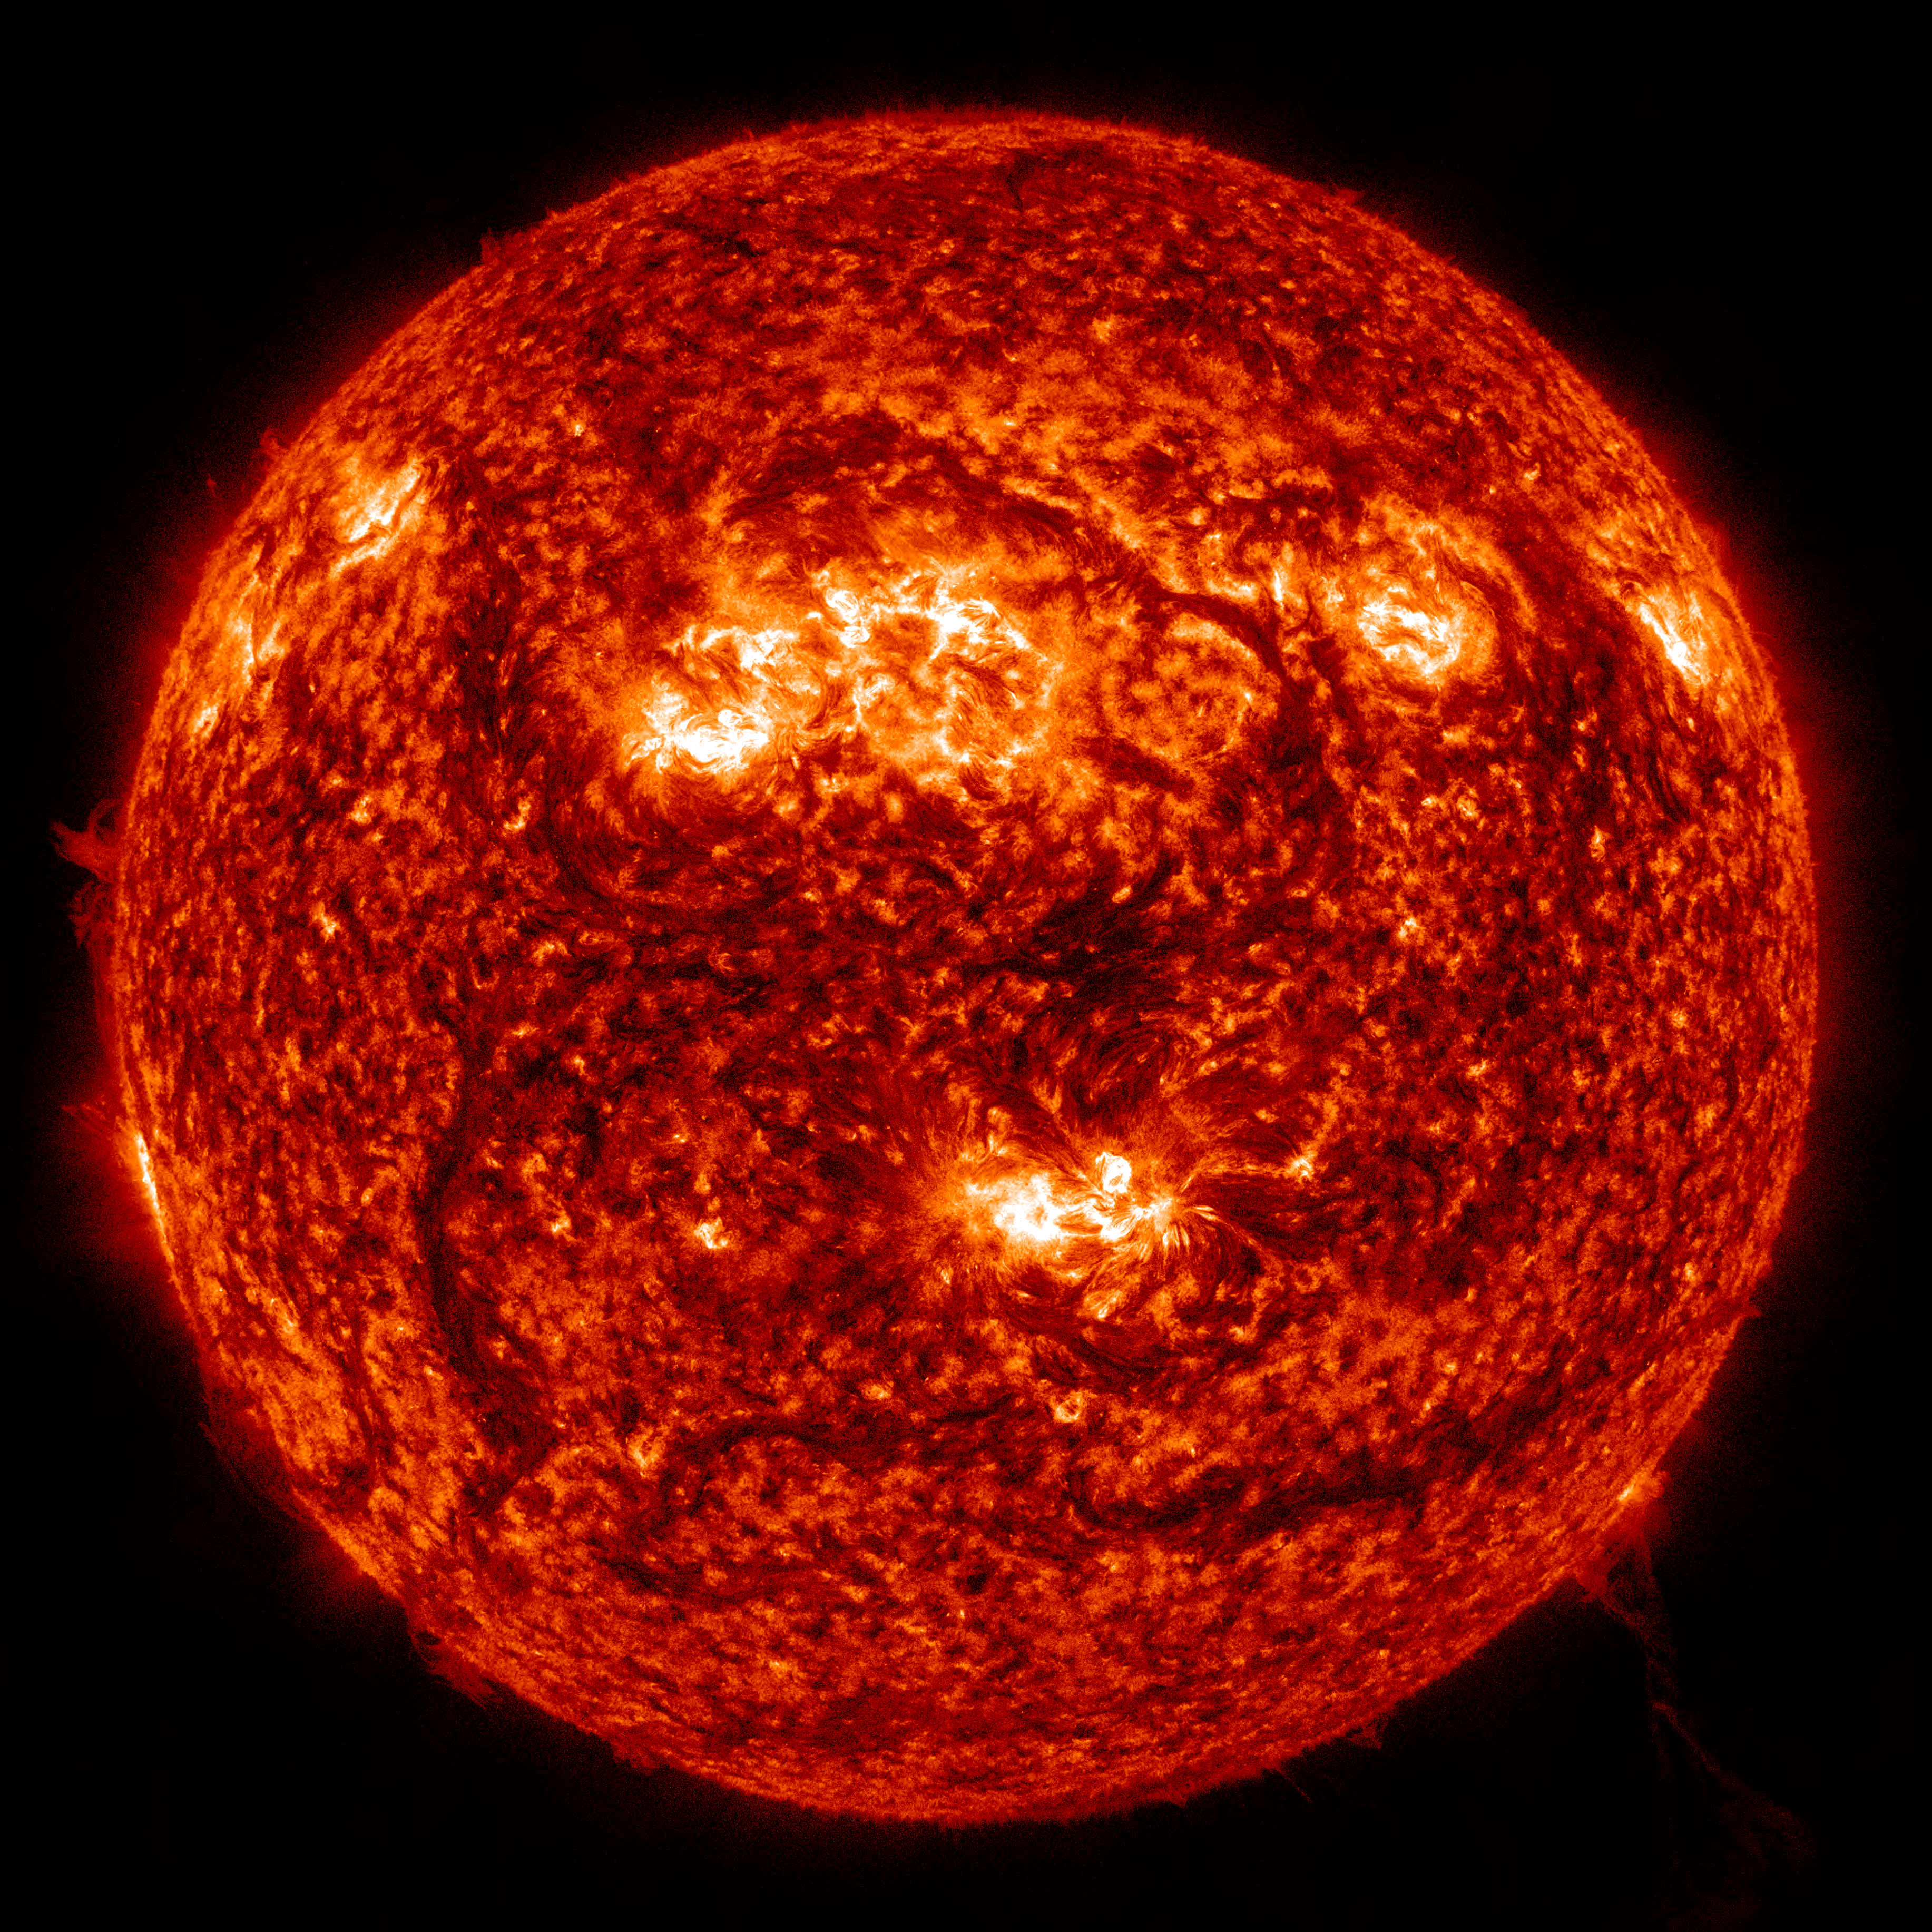
\includegraphics[width=\textwidth]{panels/panel_a_sdo.png}
        \caption{Región fuente del filamento eruptivo visto en 304~\AA{} desde SDO.}
        \label{fig:cme20221208_a}
    \end{subfigure}
    \hfill
    \begin{subfigure}[b]{0.32\textwidth}
        \centering
        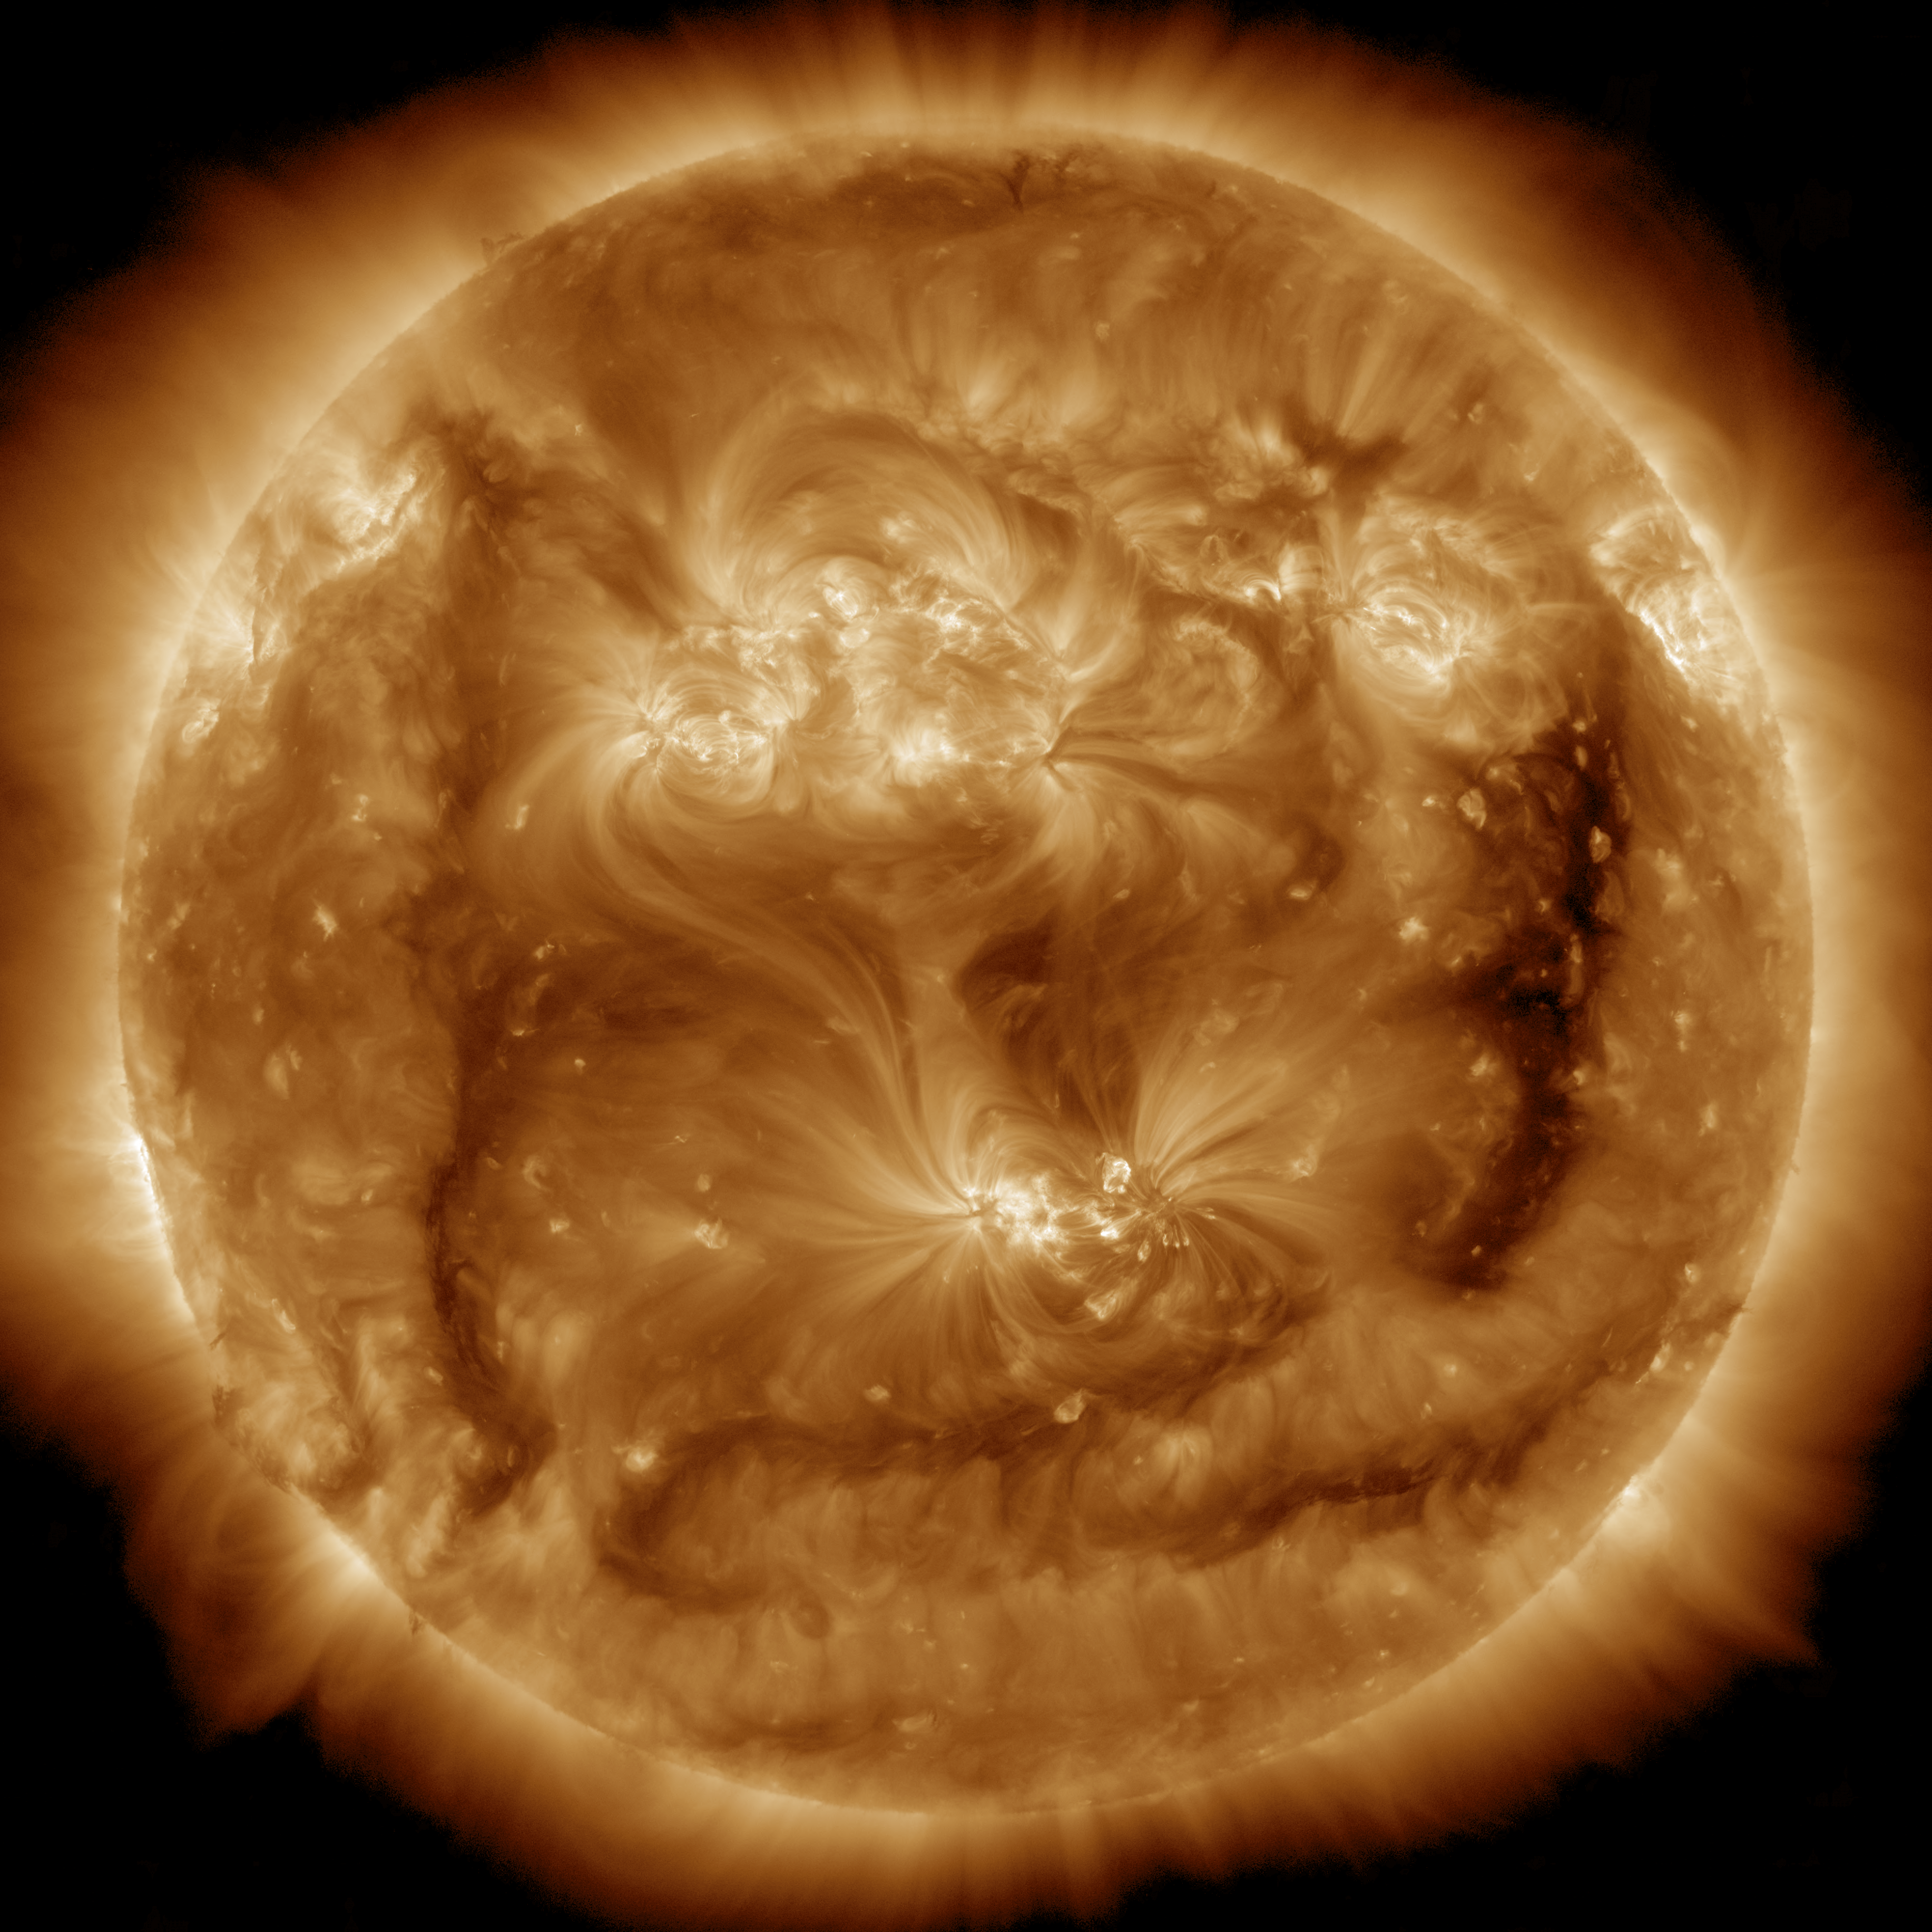
\includegraphics[width=\textwidth]{panels/panel_b_sdo.png}
        \caption{Corona baja en 193~\AA{}, mismo instante, mostrando el entorno coronal de la erupción.}
        \label{fig:cme20221208_b}
    \end{subfigure}
    \\[0.6em]
    \begin{subfigure}[b]{0.32\textwidth}
        \centering
        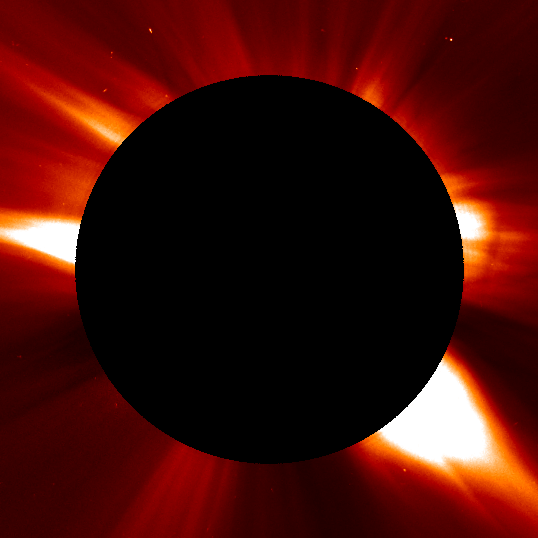
\includegraphics[width=\textwidth]{panels/panel_c_lasco c2.png}
        \caption{Primera aparición del CME en el campo de LASCO/C2 (04:12~UT).}
        \label{fig:cme20221208_c}
    \end{subfigure}
    \hfill
    \begin{subfigure}[b]{0.32\textwidth}
        \centering
        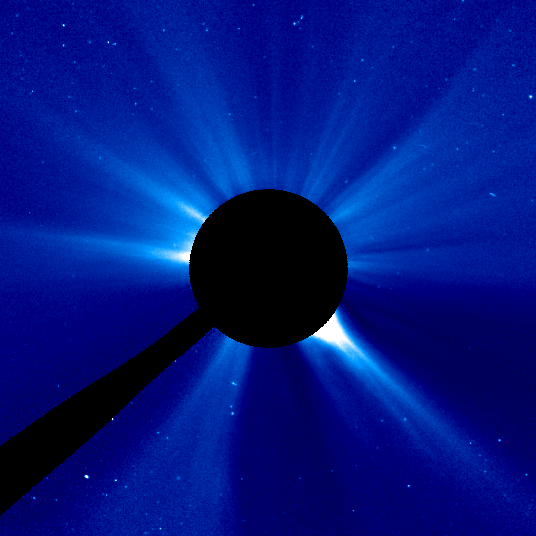
\includegraphics[width=\textwidth]{panels/panel_d_lasco c3.png}
        \caption{Estructura de halo desarrollada en LASCO/C3 (10:42~UT, PA~240\textdegree{}).}
        \label{fig:cme20221208_d}
    \end{subfigure}
    \\[0.6em]
    \begin{subfigure}[b]{0.32\textwidth}
        \centering
        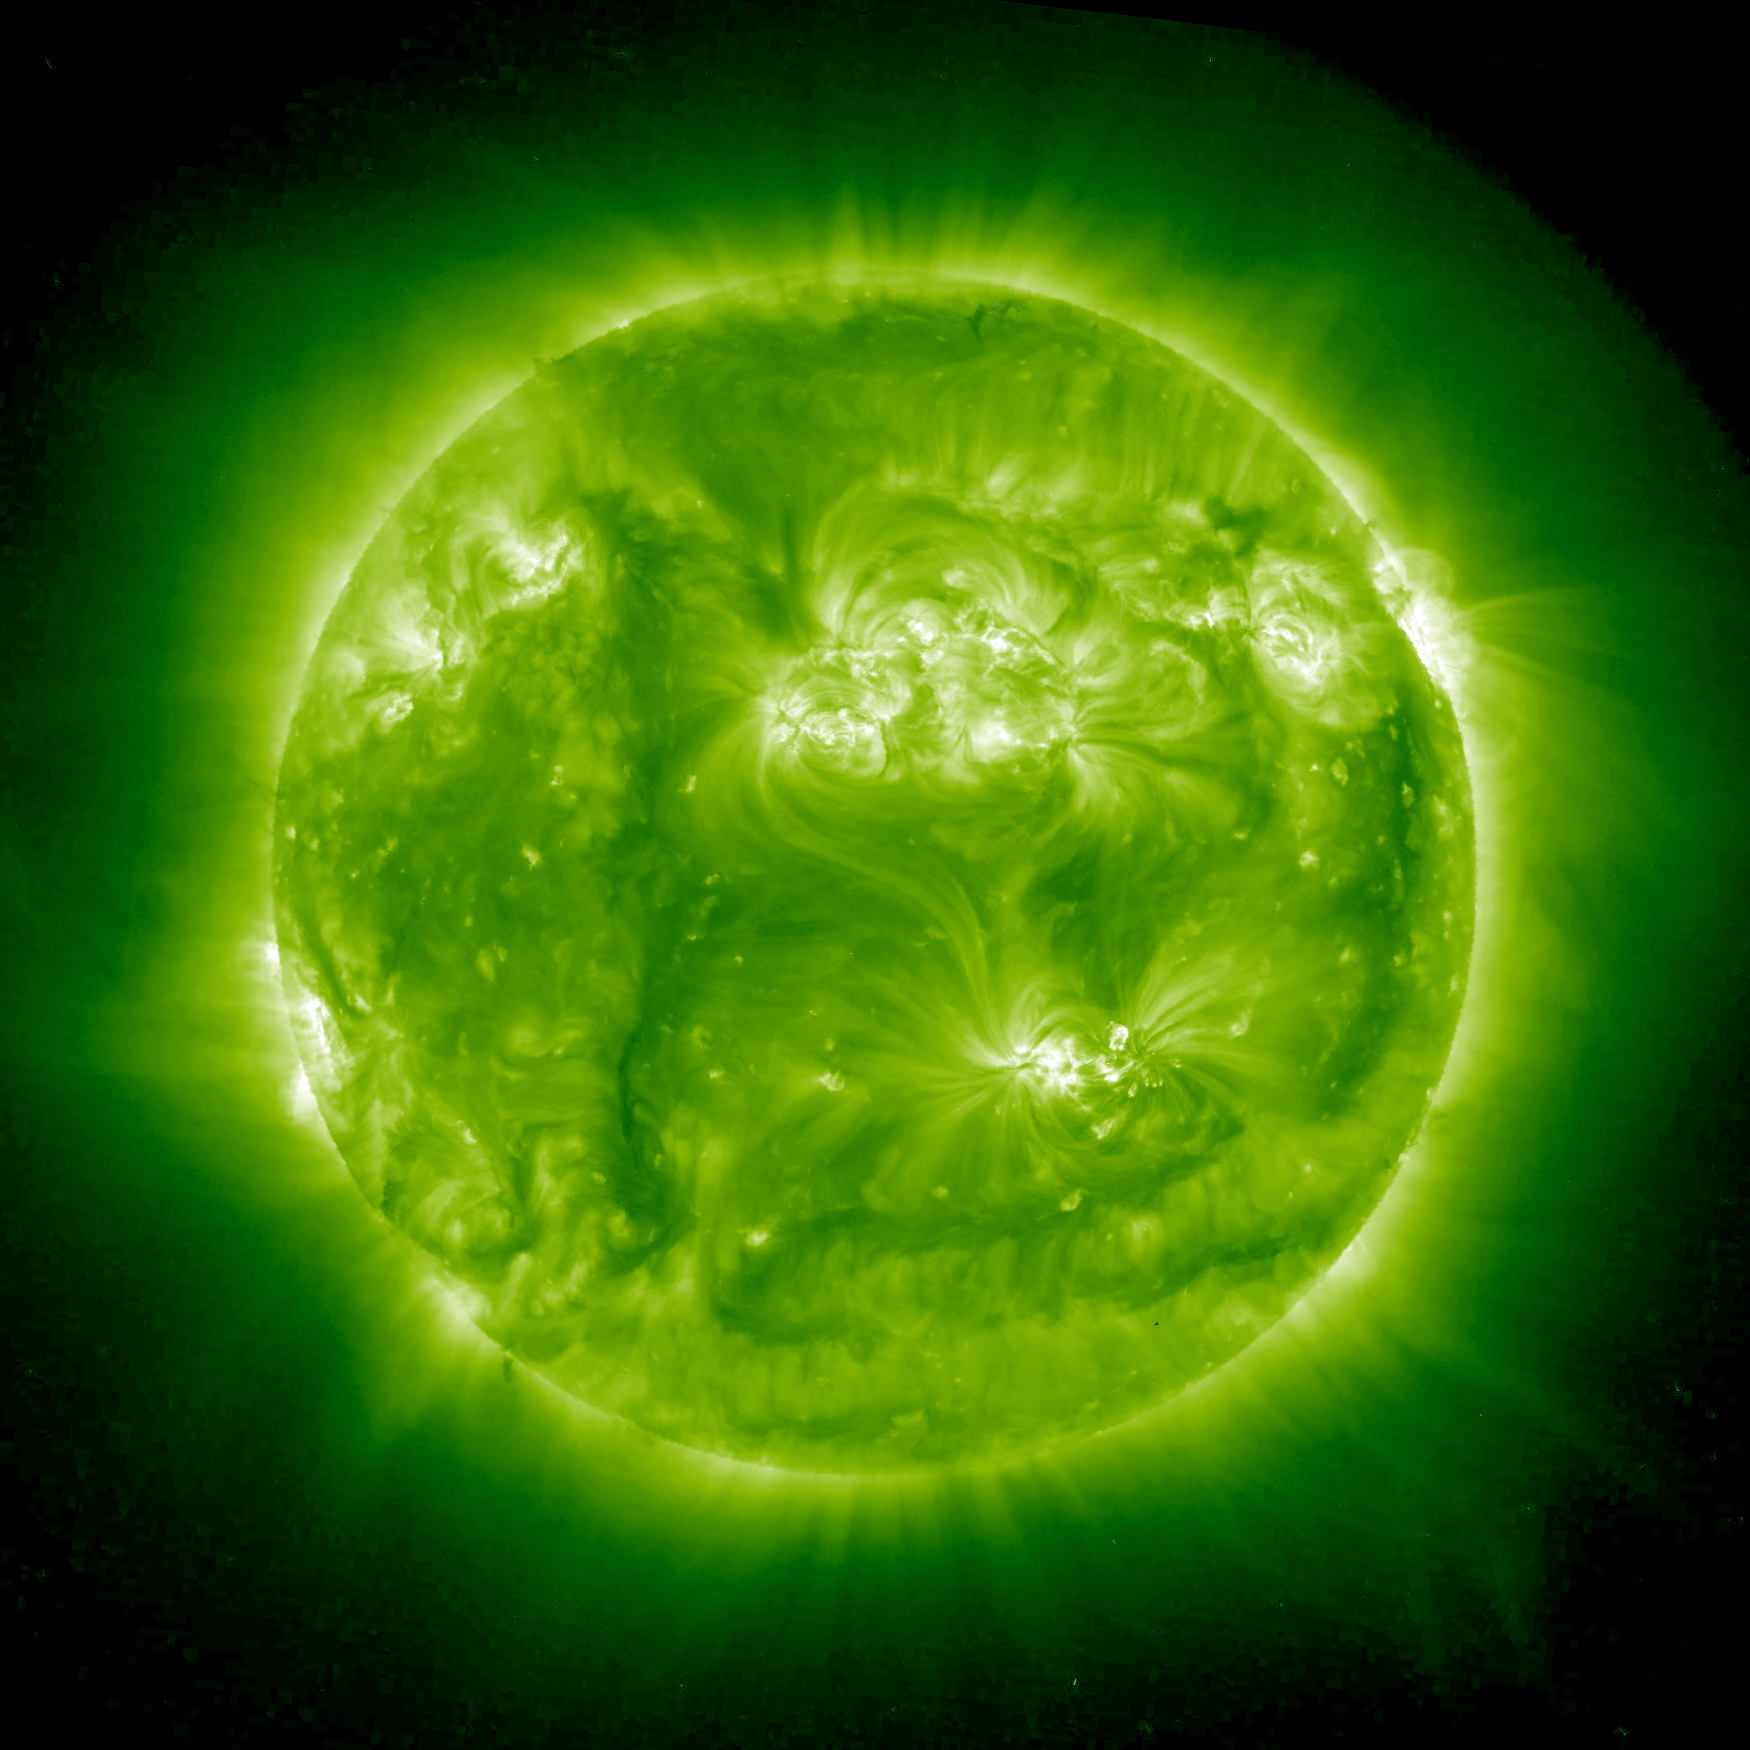
\includegraphics[width=\textwidth]{panels/panel_e_stereo-a.png}
        \caption{Vista de la región fuente desde el punto de observación de STEREO-A.}
        \label{fig:cme20221208_e}
    \end{subfigure}
    \hfill
    \begin{subfigure}[b]{0.32\textwidth}
        \centering
        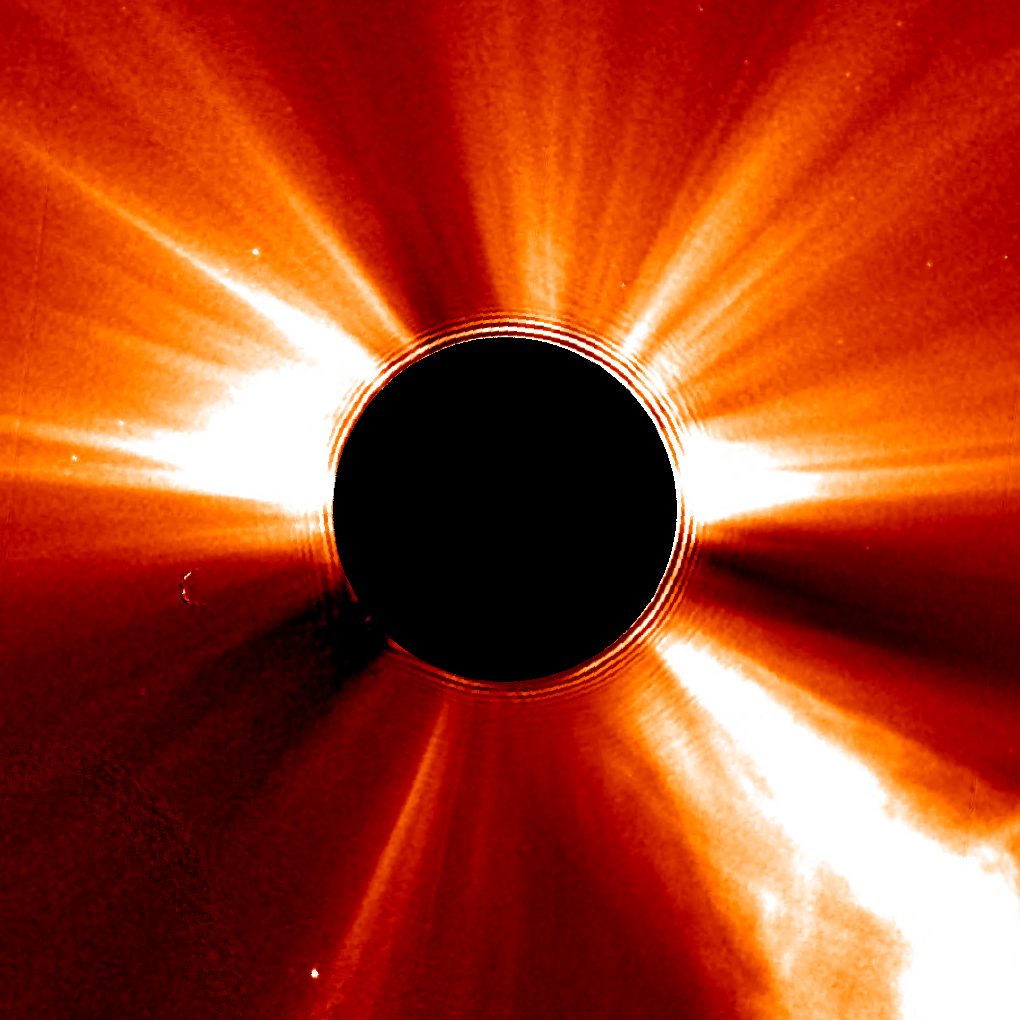
\includegraphics[width=\textwidth]{panels/panel_f_stereo-a.png}
        \caption{El mismo CME, ahora visto desde STEREO-A/COR2, evidenciando la diferencia de perspectiva respecto a SOHO.}
        \label{fig:cme20221208_f}
    \end{subfigure}
    \hfill
    \caption[CME del 8 de diciembre de 2022]{CME del 8 de diciembre de 2022, observado simultáneamente por SDO, SOHO/LASCO y STEREO-A/SECCHI. Datos obtenidos mediante la API de Helioviewer (\url{{https://api.helioviewer.org}}).}}
    \label{fig:cme20221208}
\end{figure}
